\chapter{Setting up a development environment for Open edX platform}

\section{Open edX installation options}
In order to test our local integation what we needed was a running instance of Open edX platform
on our local machine. Open edX has provided us with different installation options depending on
our use. They are described in brief below.
\begin{itemize}
	\item \textbf{Devstack:} useful if we want to modify the Open edX code. The code will be in directories
shared between the host and the guest operating systems. We should run the code in the
guest, but can edit it in the host, where we can use our own tools.
		\begin{enumerate}
		\item For Ginkgo and earlier, devstack was a Vagrant installation.
		\item For Hawthorn, devstack is based on Docker. An unsupported pre-release is
available.
		\end{enumerate}
	\item If we want to run a production installation and want a production like environemnt on our
local machne then we can use \textbf{Native} or \textbf{Manual} installation. The Native installation installs
the Open edX software on our own Ubuntu 16.04 machine in a production-like
configuration.
	\item If we want a production-like installation for testing, we can use \textbf{Fullstack} or \textbf{Native}.
Fullstack is a Vagrant instance designed for installing all Open edX services on a single
server in a production-like configuration. Fullstack is a pre-packaged Native installation
running in a Vagrant virtual machine.
\end{itemize}
Since our project deals with making changes in Open edX source code we naturally opted for Devstack, which is designed for developers

\section{Open edX Devstack}
Devstack is traditionally a Vagrant instance designed for local development. Devstack has the same system
requirements as Fullstack. This allows us to discover and fix system configuration issues early in
development. Devstack simplifies certain production settings to make development more
convenient. For example, nginx and gunicron are disabled in devstack; devstack uses Django’s
runserver instead in conformation with Open edX platform.\newline
Devstack is maintained as a set of docker containers lately and hence we chose that way as well

\section{Installing a docker based devstack}

\subsection{Prerequisites}
\begin{itemize}
	\item This installation requires Docker 17.06+ CE. It is recommended to use docker stable, but docker edge should work as well
	\item GNU-Make
	\item pip
\end{itemize}
\textbf{Note : }\newline
Linux users should not be using the \verb|overlay| storage driver. \verb|overlay2| is tested and supported, but requires kernel version 4.0+. We can check which storage driver our \verb|docker-daemon| is configured to use through following command : \newline
\begin{center}{\verb=docker info | grep -i 'storage driver'=}\end{center}

\section{Installing docker and docker compose}
Please note that, docker based devstack needs a fairly powerful computer. Our computer was using quad core core i5 7500u CPU with 8 GB RAM. Also, give more space to \verb=/= partition because docker needs more space for storing images.If you already have configured docker on your distro, you can skip this section. For following this guide, we recommend using any debian based distro where you would be able to use \verb=apt= package manager. 

\subsection{Getting docker for ubuntu}
Before we install Docker CE for the first time on a new host machine, we need to set up the Docker
repository. Afterward, we can install and update Docker from the repository. The steps are
mentioned below :
\begin{itemize}
	\item Update the \verb=apt= package index: \newline \begin{center}{\verb=$ sudo apt-get update=}\end{center}
	\item Install the packages to allow \verb=apt= to use a repository over \textbf{HTTPS}
		\newline \begin{center}{\verb=$ sudo apt-get install apt-transport-https \ =}\end{center}
		\begin{center}{\verb=ca-certificates curl software-properties-common=}\end{center}
	\item Add docker's official GPG key : \newline
		\begin{center}
		\verb=curl -fsSL https://download.docker.com/linux/ubuntu/gpg | sudo apt-key add -=
		\end{center}
		Verify that you now have the key with the fingerprint \verb=9DC8 5822 9FC7 DD38= \newline \verb=854A E2D8 8D81 803C 0EBF CD88= by searching the last 8 characters of the fingerprint\newline\newline
		\verb=$ sudo apt-key fingerprint 0EBFCD88=
		\begin{center}
			\begin{verbatim}
>> pub 4096R/0EBFCD88 2017-02-22
Key fingerprint = 9DC8 5822 9FC7 DD38 854A E2D8 8D81 803C 0EBF CD88
uid Docker Release (CE deb) <docker@docker.com>
sub 4096R/F273FCD8 2017-02-22
			\end{verbatim}
		\end{center}
	\item Use the following command to set up the \textbf{stable} repository. You always need the \textbf{stable}
repository, even if you want to install builds from the \textbf{edge} or \textbf{test} repositories as well. To
add the edge or test repository, add the word \textbf{edge} or \textbf{test} (or both) after the word 
\verb=stable= in the commands below.
		\begin{verbatim}
$ sudo add-apt-repository \
"deb [arch=amd64] https://download.docker.com/linux/ubuntu \
$(lsb_release -cs) \ stable"
		\end{verbatim}
\end{itemize}

\subsection{Installing Docker CE}
\begin{enumerate}
	\item  Update the \verb=apt= package index: \newline \begin{center}{\verb=$ sudo apt-get update=}\end{center}
	\item Install the latest version of Docker CE \newline \begin{center}{\verb=$ sudo apt-get install docker-ce=}\end{center}
	\item Docker should now be installed, the daemon started, and the process enabled to start on boot. To check that its running, we can use the following command\newline\begin{center}{\verb=$ sudo systemctl status docker=}\end{center}
\end{enumerate}

\subsection{Post installation steps for ubuntu}
\begin{enumerate}
	\item
	\textbf{Manage docker as a non root user}\newline
The docker daemon binds to a Unix socket instead of a TCP port. By default that Unix socket is
owned by the user root and other users can only access it using sudo. The docker daemon always
runs as the root user.
If we don’t want to use sudo when you use the docker command, create a Unix group called docker
and add users to it. When the docker daemon starts, it makes the ownership of the Unix socket
read/writable by the docker group.
To create the docker group and add our user:
	\begin{enumerate}
		\item Create the docker group \newline\begin{center}\verb=$ sudo groupadd docker=\end{center}
		\item Add our user to the docker group \newline\begin{center}\verb=$ sudo usermod -aG docker $USER=\end{center}
		\item Log out and log back in so that the group membership is re-evaluated. If testing on a virtual
machine, it may be necessary to restart the virtual machine for changes to take effect.\newline
On a desktop Linux environment such as X Windows, we need to log out of our session
completely and then log back in.
		\item Verify that you can run docker commands without sudo.\newline\begin{center}\verb=$ docker run hello-world=\end{center}
			This command downloads a test image and runs it in a coontainer. When the container runs, it prints an informational message and exits.
	\end{enumerate}

	\item
	\textbf{Configure Docker to start on boot}\newline
Most current Linux distributions (RHEL, CentOS, Fedora, Ubuntu 16.04 and higher) use \verb=systemd=
to manage which services start when the system boots. Ubuntu 14.10 and below use \verb=upstart=.
	\begin{enumerate}
	\item \verb=systemd= \newline\begin{center}\verb=$ sudo systemctl enable docker=\end{center}
		To disable this behavior, use \verb=disable= instead\newline
		\begin{center}\verb=$ sudo systemctl disable docker=\end{center}
	\item \verb=upstart= \newline
		Docker is automatically configured to start on boot using \verb=upstart=. 
		To disable this behavior, use the following command \newline
		\begin{center}\verb=$ echo manual | sudo tee /etc/init/docker/override=\end{center}
	\end{enumerate}
	\verb=chkconfig=
	\begin{center}\verb=$ sudo chkconfig docker on=\end{center}
\end{enumerate}

\subsection{Getting Docker compose for ubuntu}
On \textbf{Linux}, you can download the Docker Compose binary from the Compose repository page on git
hub. These step by step instructions are also included below.
\begin{enumerate}
	\item Run this command to download latest version of docker compose:
		\begin{center}
		\begin{verbatim}
		sudo curl -L
https://github.com/docker/compose/releases/download/1.21.2/docker-compose-
$(uname -s)-$(uname -m) -o /usr/local/bin/docker-compose
		\end{verbatim}
		\end{center}
		We should use the lates compose release number in download command. The above command is an example and it may become out-of-date. To ensure you have the latest version, check the compose repository on release page on GitHub \url{https://github.com/docker/compose/releases}
		\newline If you have problems installing with \verb=curl=, you can find alternative options in docker documentation.
	\item Apply the executable permissions to the binary\newline\begin{center}\verb=$ sudo chmod +x /usr/local/bin/docker-compose=\end{center}
	\item Test the installation
		\begin{center}
		\begin{verbatim}
$ docker-compose –version
>>docker-compose version 1.21.2, build 1719ceb
		\end{verbatim}
		\end{center}
\end{enumerate}

\section{Installing docker based devstack}
\begin{enumerate}
	\item Clone the git repository of devstack\newline
	\begin{center}
	\begin{verbatim}$ git clone https://github.com/edx/devstack && cd devstack
	\end{verbatim}
	\end{center}
	\item Install the requirements inside of a python virtualenv \newline
	\begin{center}
	\begin{verbatim}$ make requirements
	\end{verbatim}
	\end{center}
	\item The Docker Compose file mounts a host volume for each service's executing code. The
host directory defaults to be a sibling of this directory. For example, if this repo is
cloned to \verb=~/workspace/devstack=, host volumes will be expected in \verb=~/workspace/coursediscovery=,
\verb=~/workspace/ecommerce=, etc. These repos can be cloned with the command
below.\newline
\begin{center}
\begin{verbatim}make dev.clone
\end{verbatim}
\end{center}
We may customize where the local repositories are found by setting the
\verb=DEVSTACK_WORKSPACE= environment variable
	\item We must Run the provision command, if we haven't already, to configure the various
services with superusers (for development without the auth service) and tenants (for multitenancy).
When running the provision command, databases for ecommerce and edxapp will
be dropped and recreated.
The username and password for the superusers are both edx. We can access the services
directly via Django admin at the \verb=/admin/= path, or login via single sign-on at \verb=/login/=.\newline
\begin{center}
Default: \verb=make dev.provision=
\end{center}
	\item Start the services. This command will mount the repositories under the
\verb=DEVSTACK_WORKSPACE= directory. It may take up to 60 seconds for the LMS to start,
even after the \verb=make dev.up= command outputs done.\newline
\begin{center}
Default: \verb=make dev.up=
\end{center}
\end{enumerate}

Please note that all the above commands are to be executed in \verb=devstack= directory and \verb=DEVSTACK_WORKSPACE= MUST be exported correctly throughout the process.

After the services have started, if we need shell access to one of the services, we can run \begin{verbatim}make <service>-shell\end{verbatim}. For example to access the Catalog/Course Discovery Service, we can run:\newline
\begin{center}
\verb=make discovery-shell=
\end{center}
To see logs from containers running in detached mode, we can either use "Kitematic" (available
from the "Docker for Mac" menu), or by running the following:\newline
\begin{center}
\verb=make logs=
\end{center}
The screenshots of the running instance of our Devstack along with the LMS and CMS
section are provided as mentioned below:
\begin{center}
\textbf{[See Figures 5-8 in the “Figures and Screenshots” section.]}
\end{center}

\subsection{Service URLs}
Each service is accessible at \verb=localhost= on a specific port. The table below provides links
to the homepage of each service. Since some services are not meant to be user-facing, the
"homepage" may be the API root
\begin{center}
	\begin{tabular}{ |c|c| }
	\hline
	\textbf{Service} & \textbf{URLs} \\
	\hline
	Credentials & http://localhost:18150/api/v2/ \\
	Catalog/Discovery & http://localhost:18381/api-docs/ \\
	E-commerce/Otto & http://localhost:18130/dashboard/ \\
	LMS & http://localhost:18000/ \\
	Notes/edx-notes-api & http://localhost:18150/api/v1/ \\
	Studio/CMS & http://localhost:18010 \\
	\hline
	\end{tabular}
\end{center}

\section{Why OpenEdx might have moved to a docker based installation ?}
In vagrant based installation, the images are being provided by virtualbox which in trun slows
down the performance of the system. On the other hand docker uses containers for
virtualizing andt this is a vast difference in approaches.\newline
In a docker container, the image contains only the data it needs and the rest of the
data/packages are installed on/fetched from host machine which dramatically improves
performance. Also in docker based devstack, each service has it’s own dedicated container
which is accessible through machine. This makes the developer’s access to each service
individually very easy which in turn speeds up debugging and development rate.\newline

\section{Issues and solutions}
During the course of our Docker based installation and configuration of Open edX Devstack,
we faced multipled issues such as poxy settings etc. The issues are mentioned below along
with the solutions we used to overcome them.
\begin{enumerate}
	\item \textbf{Proxy configuration of the system :}\newline
		\begin{itemize}
		\item Initially we tried installing our instance of Open edX Devstack behind a proxy server. But
many packages mainly the ones which were being installed using pip were failing.
		\item We thought of trying to enable proxy inside the docker container, but due to the large
amount of time it took to resolve several layers of proxy authentication the reuqest was
getting timed out.
		\item Thus, the docker container was unable to fetch the required packages from Open edX.
		\end{itemize}
		\textbf{Solution :}After trying several times, we decided to discard the installation using a proxy.
We used normal mobile data to install all the require services and get our Devstack up and
running. With the help of mobile data the installation was completed error free and all the
packages were downloaded correctly.
	\item \textbf{Issue with docker installation : }\newline
		Docker isntallation can create some problems if the steps are not followed correctly and in
order. After installing Docker it is important to perform the post installation steps ,
because it happens sometimes that the system is unable to connect to the docker daemon.
	\item \textbf{Issues compiling static assets : }\newline
This is a package related issue. This can happen with any of the service randomly. The issue here is
the script that is building static assets for a particular service, needs only a specific version of npm
package “babel-loader”. Sometimes durirng the provisioning, it updates the package “babel-loader”
via npm. We could not exactly find out when the update was happening, it was random most of the
times. If you ever encounter issue with newer “babel-loader”, just modify the webpack to explicitly
tell the “babel-loader” to build JSX as ReactNative assets. Also it might give error about Object
Spread, all you need to do it to add plugin into your webpack\newline
The modified webpack can be found on our git\newline
Also check out :\newline

\begin{small}\url {https://stackoverflow.com/questions/33460420/babel-loader-jsx-syntaxerror-unexpected-token}\end{small} \& \newline
\begin{small}\url{https://babeljs.io/docs/en/babel-plugin-transform-object-rest-spread}\end{small}
	\item \textbf{Docker environment issues :} \newline
	\begin{figure}
		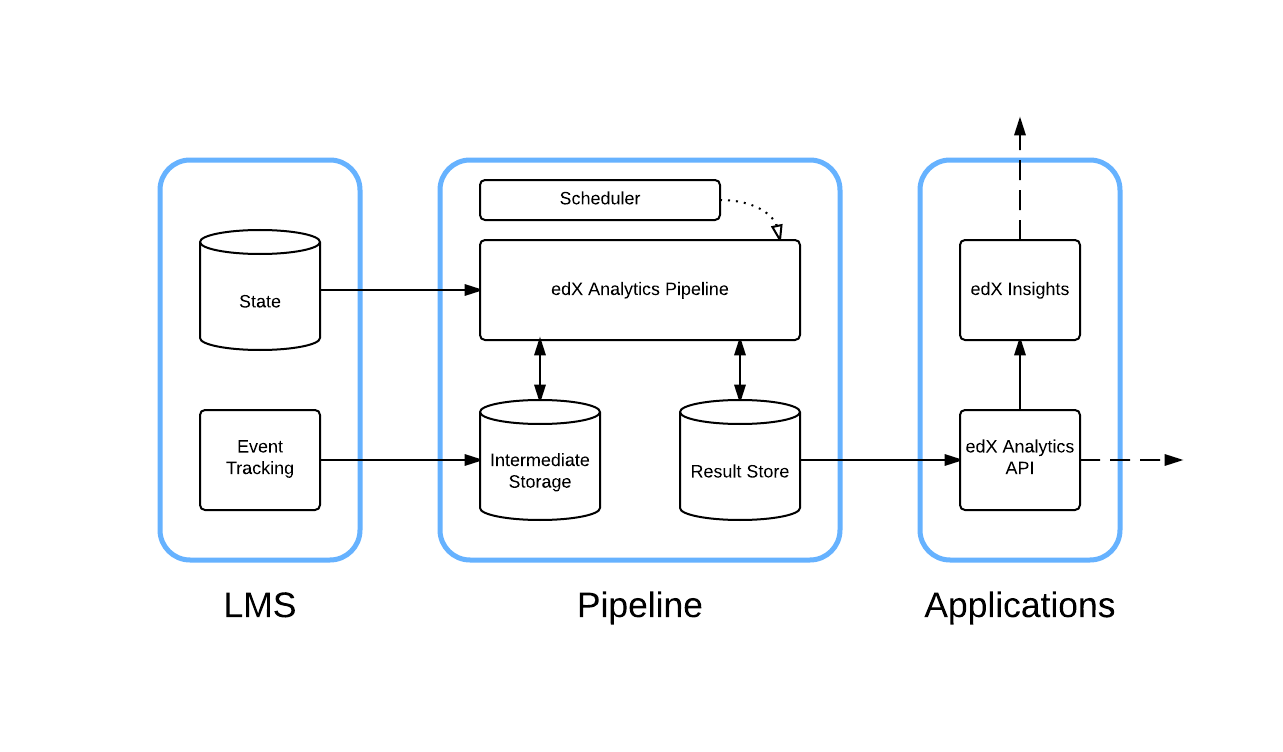
\includegraphics[width=\linewidth]{images/devstack_arch.png}
		\caption{Block diagram of devstack service}
	\end{figure}
As we can see in the diagram, every devstack service is made up of docker image and docker
volume. Docker images are pulled from openedx repos whereas volumes are mounted on your host
device. While mounting these docker volumes, script uses an environment variable called 
\verb=DEVSTACK_WORKSPACE= as shown in figure. It is highly probable that you set this variable
once and when retrying we forget to set this variable again. If we donot set this variable correctly
the mount silently fails and mounts a new volume instead. This is why it is necessary to set this
variable everytime you login into your host machine. For doing so, add the 
	\begin{center}
	\begin{verbatim}"export DEVSTACK_WORKSPACE=/path/to/your/workspace"
	\end{verbatim}
	\end{center} line at the bottom of your \verb=.bashrc.=
After doing “\verb=source .bashrc=” will export the variable correctly. To see whether the variable is set
correctly or not, type “\verb=printenv=”\newline
Important note for “sudo”. If you are doing any command with sudo, make sure to preserve the
current environment variables. For doing so, use -E flag with sudo to preserve them.
	
	
\end{enumerate}
